\chapter[Higher order matching (BLT)]{Higher-order matching in Boundary Layer Theory}
Several ways to match. No set way!

\paragraph{Example 1:} Consider
\begin{gather}
	\epsilon y'' + (1+x)y' + y = 0 \label{eqn:wk13-ode}\\
	y(0) = 0 \qquad y(1) = 1 \nonumber
\end{gather}
Such problems where $\epsilon$ multiplies the highest derivative typifies ``singular'' problems. We will learn techniques in the next lecture which will help us identify the thickness and other characteristics of the BL. For this problem the BL is at $x=0$ and has thickness $O(\epsilon)$. 

\paragraph{Outer soln.} Try the regular perturbation series
\begin{gather*}
	y = y_0 + \epsilon y_1 + O(\epsilon^2)
\end{gather*}
We can first rewrite the ODE as
\begin{gather*}
	\epsilon y'' + [(1+x)y]' = 0
\end{gather*}
The $O(\epsilon^0)$ solution can be written directly
\begin{gather*}
	(1+x)y_0 = a
\end{gather*}
At $O(\epsilon^1)$
\begin{align*}
	[(1+x)y_1]' &= -y_0'' \\
		(1+x)y_1 &= -y_0' + b 
\end{align*}
which yields
\begin{gather*}
	y_1 = \frac{a}{(1+x)^3} + \frac{b}{(1+x)}
\end{gather*}
The outer solution will use the BC at $x=1$
\begin{gather*}
	y(1) = y_0(1) + \epsilon y_1(1) + \dots = 1 + 0\epsilon + \dots 
\end{gather*}
which determines both constants:
\begin{gather*}
	y(x,\epsilon) = \frac{2}{1+x} + \epsilon \left[\frac{2}{(1+x)^3} - \frac{1}{2(1+x)}\right] + O(\epsilon^2)
\end{gather*}
\paragraph{Inner soln.} Let us scale the problem by introducing $X = x/\epsilon$. 
\begin{gather*}
	Y'' + (1+\epsilon X) Y' + \epsilon Y = 0
\end{gather*}
And use regular perturbation method since we will no longer lose the highest derivative
\begin{gather*}
	Y = Y_0 + \epsilon Y_1 + O(\epsilon^2) \\
	Y(0) = 0 + 0\epsilon + \dots = Y_0 + \epsilon Y_1 + \dots 
\end{gather*}
Substituting
\begin{gather*}
	(Y_0'' + \epsilon Y_1'' + \dots ) + (1+\epsilon X)(Y_0' + \epsilon Y_1'+\dots) + \epsilon (Y_0 + \epsilon Y_1 + \dots ) = 0
\end{gather*}
This leads to
\begin{align*}
	O(\epsilon^0): \qquad &Y_0'' + Y_0' = 0 \\
	O(\epsilon^1): \qquad &Y_1'' + Y_1' = -XY_0' - Y_0
\end{align*}
At $O(\epsilon^0)$, we integrate once and then use the integrating factor method to solve the first order ODE with the BCs
\begin{gather*}
	Y_0(X) = A(1-\me^{-X})
\end{gather*}
Our $O(\epsilon^1)$ equation reads
\begin{gather*}
	Y_1'' + Y_1' = -AX\me^{-X} - A(1-\me^{-X})
\end{gather*}
Proceed by integrating both side
\begin{align*}
	Y_1' + Y_1 &= A (X\me^{-X}+\cancel{\me^{-X}}) - A(X + \cancel{\me^{-X}}) + B
\end{align*}
The integrating factor method yields
\begin{align*}
	Y_1 \me^X &= \int \me^X [AX\me^{-X} - AX + B] \md X \\
	&= \int [AX - AX\me^X + B\me^X] \md X \\
	&= \frac{1}{2}AX^2 - A[X\me^X - \me^X + C] + B\me^X  \\
	Y_1 &= \frac{1}{2}AX^2 \me^{-X} - A(X-1) -AC\me^{-X} + B \\
	&= AX\left(\frac{1}{2}X\me^{-X} - 1\right) + \underbrace{A+B - AC\me^{-X}}_{E(1-\me^{-X})?}
\end{align*}
\paragraph{Intermediate region matching:} The simplest, or ``primitive'' matching (given by Prandtl) is the lowest order match. 
\begin{align*}
	\lim\limits_{X\rightarrow \infty}Y_0(X) &= \lim\limits_{x \rightarrow 0} y_0(x) \\
	A &= 2
\end{align*}
Then our composite solution would be
\begin{align}
	y_c(x) &= Y_\text{inn} + y_\text{out} - y_\text{match} \nonumber \\
	&= 2(1-\me^{-x/\epsilon}) + \frac{2}{1+x} - 2 \nonumber \\
	&= 2\left[\frac{1}{1+x} - \me^{-x/\epsilon}\right] \label{eqn:wk13-ana-low-order}
\end{align}
{\bf NB.} In the higher order match, $y_\text{match}$ may be a function and not a number. {\color{red} [To do]} Use Wronskian method too? 
\begin{figure}[!h]
	\centering
	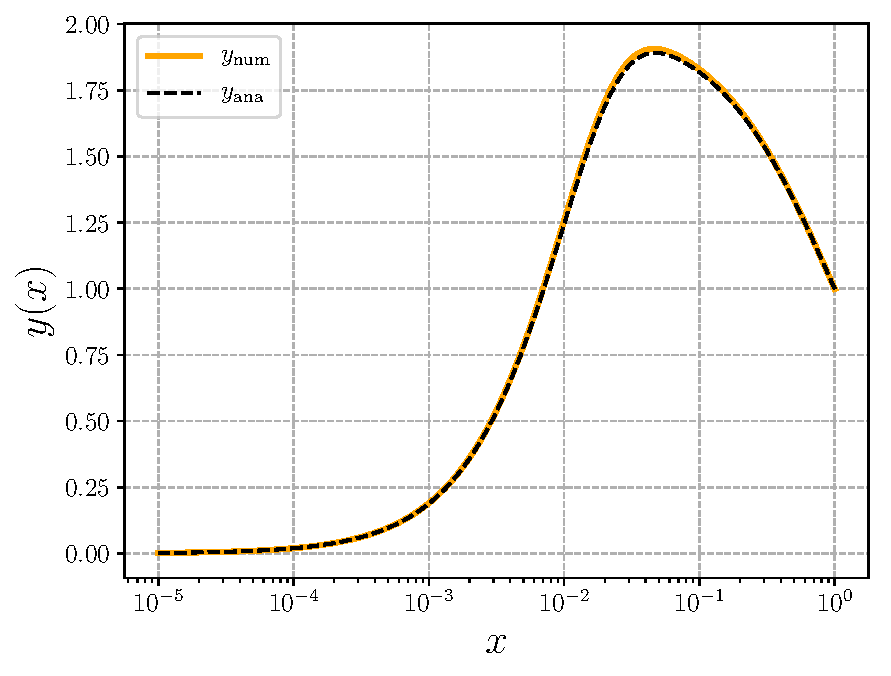
\includegraphics[width=0.65\textwidth]{./plots/pdf/strogatz-wk13.pdf}
	\caption{Solving eqn. \ref{eqn:wk13-ode} in Python using the \texttt{scipy.integrate.solve\_bvp} module along with the $O(\epsilon^0)$ composite solution given by eqn. \ref{eqn:wk13-ana-low-order}.}
	\label{fig:strogatz-wk13}
\end{figure} \\
In the higher order match, noting that $\epsilon \rightarrow 0^+$ and $x \rightarrow 0$, we keep terms of $O(x,\epsilon)$ and discard terms of $O(x^2, \epsilon x, \epsilon^2)$. Going to a still higher order, we would discard $O(x^3,\epsilon^3)$ terms. Note that the implicit assumption is
\begin{gather*}
	x^2 \ll \epsilon
\end{gather*}
B\&O mention that at each higher order of matching, the matching region gets smaller and smaller. The ordering
\begin{gather*}
	\epsilon \ll x \ll \epsilon^{1/2}
\end{gather*}
emerges since the overlap region is multiple $\epsilon$ to the right of the left boundary. Contrast this with the $O(\epsilon^0)$ overlap region
\begin{gather*}
	\epsilon \ll x \ll 1
\end{gather*}
Expanding the outer solution for small $x,\epsilon$:
\begin{align*}
	y_\mathrm{out} &= \frac{2}{1+x} + \epsilon \left[\frac{2}{(1+x)^3}-\frac{1}{2(1+x)}\right] + O(\epsilon^2)\\
	&= 2 [1-x + O(x^2)] + \epsilon [2(1-3x) - (1-x)/2] + O(\epsilon^2) \\
	&= 2(1-x) + \frac{3}{2}\epsilon + O(x^2,\epsilon x, \epsilon^2)
\end{align*}
Similarly for the inner region, $X\gg 1$, but again, $O(\epsilon^2 X^2, \epsilon^2, \epsilon^2 X)$ terms are neglected
\begin{align*}
	Y_\mathrm{inn} &= 2(1-\me^{-X}) + \epsilon \left[ 2X\left(\frac{1}{2}X\me^{-X} - 1\right) + {E(1-\me^{-X})}\right] + O(\epsilon^2) \\
	&= 2 + \epsilon \left[-2X + E\right] + O(\epsilon^2) + \mathrm{TST} \\
	&= 2 - 2x + \epsilon E 
\end{align*}
Now the inner and outer solutions match for 
\begin{gather*}
	E = \frac{3}{2}
\end{gather*}
and
\begin{align*}
	y_\mathrm{match} = 2 - 2x + \frac{3}{2}\epsilon + \dots 
\end{align*}